\section{Implémentation \texttt{VHDL} du \texttt{GCD}}
% =====================================================================
\begin{frame}[fragile,t]{FSMD : interconnexion contrôleur / chemin de données}
\begin{columns}[T]
\begin{column}{0.54\textwidth}
\codecap{fsmd.vhd}
\begin{lstlisting}
entity fsmd is
  ...
end entity;
architecture rtl of fsmd is
  signal |controls_s| : control_type;
  signal |status_s| : status_type;
begin
  controler_i: entity gcd_lib.controler
  port map (
    ...
    go       => go,
    done     => done,
    controls => |controls_s|,
    status   => |status_s|
  );
  datapath_i: entity gcd_lib.datapath
  port map (
    ...
    data     => data,
    result   => result,
    controls => |controls_s|,
    status   => |status_s|
  );
end rtl;
\end{lstlisting}
\end{column}
\begin{column}{0.44\textwidth}
\fig[62mm]{fig1_fsmd}
\end{column}
\end{columns}
\takeaway{Pur câblage structurel (aucune logique dans \texttt{fsmd}) ; deux types enregistrement de \texttt{type\_pkg} servent d'interface.}
\end{frame}

% =====================================================================
\begin{frame}[fragile,t]{Un registre du chemin de données : \texttt{reg\_a}}
\begin{columns}[T]
\begin{column}{0.54\textwidth}
\codecap{datapath.vhd}
\begin{lstlisting}
constant READ_DATA : integer range 0 to 2 := 1;
constant SAMPLE_COMPUTED_VALUE : integer range 0 to 2 := 2;
signal reg_a,reg_b, computed_value : unsigned(31 downto 0);
...
reg_a_p : process(reset_n,clk)
begin
  if reset_n='0' then
    reg_a <= to_unsigned(0,32);
  elsif rising_edge(clk) then
    case |controls.cmd_1| is
      when READ_DATA =>
        reg_a <= |data|;
      when SAMPLE_COMPUTED_VALUE =>
        reg_a <= |computed_value|;
      when others =>
        null;   -- maintien
    end case;
  end if;
end process;
...
result <= reg_a;
\end{lstlisting}
\end{column}
\begin{column}{0.44\textwidth}
\fig[62mm]{fig2_reg_a}
\end{column}
\end{columns}
\takeaway{3 comportements pilotés par \texttt{cmd\_1} : maintenir, lire \texttt{data}, échantillonner le résultat ; \texttt{reg\_b} est identique avec \texttt{cmd\_2}.}
\end{frame}

% =====================================================================
\begin{frame}[fragile,t]{Cœur de calcul : conditions et soustraction}
\begin{columns}[T]
\begin{column}{0.50\textwidth}
\codecap{datapath.vhd}
\begin{lstlisting}
arg_1 <= reg_a when |controls.cmd_3|=0 else reg_b;
arg_2 <= reg_a when |controls.cmd_4|=0 else reg_b;
computed_value <= arg_1 - arg_2;
status.a_gt_b  <= reg_a > reg_b ;
status.a_neq_b <= reg_a /= reg_b ;
\end{lstlisting}
\vspace{1.5mm}
\codecap{controler.vhd}
\begin{lstlisting}
when COMPUTE =>
  if |status.a_neq_b| then
    if |status.a_gt_b| then
      controls_c.cmd_3 <= 0;--arg1=a
      controls_c.cmd_4 <= 1;--arg2=b
      controls_c.cmd_1 <= 2;--sample result
    else
      controls_c.cmd_3 <= 1;--arg1=b
      controls_c.cmd_4 <= 0;--arg2=a
      controls_c.cmd_2 <= 2;--sample result
    end if;
  else
    done_c <= '1';
    state_c <= IDLE;
  end if;
\end{lstlisting}
\end{column}
\begin{column}{0.48\textwidth}
\fig[62mm]{fig3_calcul}
\end{column}
\end{columns}
\takeaway{Euclide par soustractions : $a>b \Rightarrow a\leftarrow a-b$, $a<b \Rightarrow b\leftarrow b-a$, $a=b \Rightarrow$ \texttt{done}.}
\end{frame}

% =====================================================================
\begin{frame}[fragile,t]{Protocole d'utilisation : \texttt{go}, puis \texttt{a} et \texttt{b} sur \texttt{data}}
  \begin{columns}[T]
    \begin{column}{0.40\textwidth}
      \codecap{fsmd\_tb.vhd}
      \begin{lstlisting}
      toggle(go);  -- impulsion de 1 cycle
      data <= to_unsigned(48,32);  -- a
      wait_cycles(1);
      data <= to_unsigned(18,32);  -- b
      wait_cycles(200);
      \end{lstlisting}
      \vspace{1.5mm}
      \codecap{controler.vhd}
      \begin{lstlisting}
      when IDLE =>
        if go='1' then
          state_c <= READ_A;
        end if;
      when READ_A =>
        controls_c.cmd_1 <= 1;  -- reg_a <= data
        state_c <= READ_B;
      when READ_B =>
        controls_c.cmd_2 <= 1;  -- reg_b <= data
        state_c <= COMPUTE;
      \end{lstlisting}
      \vspace{1.5mm}

      {\footnotesize
      \begin{enumerate}\setlength\itemsep{0pt}
        \item \texttt{go} à 1 pendant un cycle
        \item \texttt{a} sur \texttt{data} (\texttt{READ\_A})
        \item \texttt{b} sur \texttt{data} (\texttt{READ\_B})
        \item attendre \texttt{done} ; lire \texttt{result}
      \end{enumerate}}

    \end{column}

    \begin{column}{0.58\textwidth}
      \fig[62mm]{fig4_chrono}
    \end{column}
  \end{columns}
\end{frame}

% =====================================================================
\begin{frame}[fragile,t]{Architecture du banc de test}
  \begin{columns}[T]
    \begin{column}{0.54\textwidth}
    \codecap{fsmd\_tb.vhd}
    \begin{lstlisting}
    entity fsmd_tb is
    end entity;
    architecture bhv of fsmd_tb is
      constant HALF_PERIOD : time :=5 ns;
      signal clk : std_logic := '0';
      signal running : boolean := true;
      procedure wait_cycles(n : natural) is ...
      procedure toggle(signal s : inout std_logic) is ...
      ...
    begin
      |reset_n| <= '0','1' after 123 ns;
      |clk| <= not(clk) after HALF_PERIOD when running else clk;
      |dut| : entity work.fsmd(rtl)
        port map (
          ...
        );
      |stim| : process
      begin
        wait until reset_n='1';
        ...
        running <= false;
        wait;
      end process;
    end bhv;
    \end{lstlisting}
    \end{column}

    \begin{column}{0.44\textwidth}
      \fig[62mm]{fig5_testbench}
    \end{column}
  \end{columns}
  \takeaway{Testbench sans port : horloge, reset, DUT et processus de stimuli ; pas d'\texttt{assert}, on vérifie \texttt{result} (= 6) au chronogramme.}
\end{frame}

\begin{frame}{Résultats de simulation VHDL}
  \begin{center}
    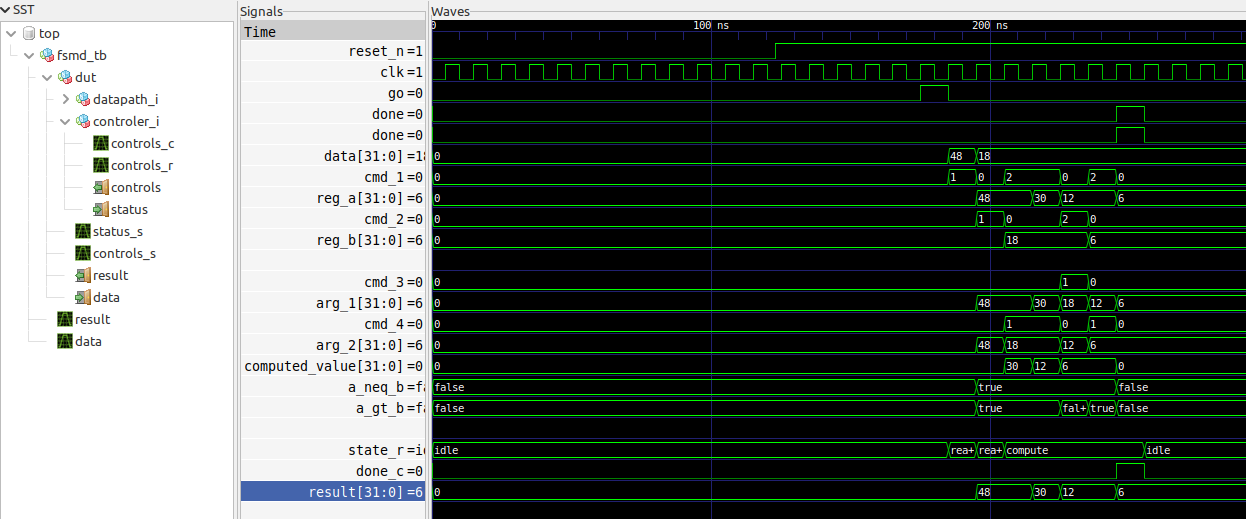
\includegraphics[scale=0.3]{./images/gcd_gtkwave.png}
  \end{center}
\end{frame}

\begin{frame}[fragile,t]{Script de simulation :  GHDL + GTKWave}
  \begin{columns}[T]
    \begin{column}{0.52\textwidth}
    \codecap{compile.x}
    \begin{lstlisting}[style=shell]
    echo "=> cleaning"
    rm *.cf

    echo "=> compiling RTL files"
    ghdl @-a@ --work=gcd_lib type_pkg.vhd
    ghdl @-a@ --work=gcd_lib controler.vhd
    ghdl @-a@ --work=gcd_lib datapath.vhd
    ghdl @-a@ --work=gcd_lib fsmd.vhd

    echo "=> compiling testbench"
    ghdl @-a@ --work=gcd_lib fsmd_tb.vhd

    echo "=> elaboration"
    ghdl @-e@ --work=gcd_lib fsmd_tb

    echo "=> running simulation"
    ghdl @-r@ --work=gcd_lib fsmd_tb --wave=top.ghw

    echo "=> opening waveform viewer"
    gtkwave top.ghw top.sav
    \end{lstlisting}
    \end{column}

    \begin{column}{0.46\textwidth}
      \fig[64mm]{fig6_compile}
    \end{column}
  \end{columns}
  \takeaway{Tout est compilé dans la bibliothèque \texttt{gcd\_lib} (\texttt{-{}-work}) : \texttt{type\_pkg} d'abord, \texttt{fsmd} après ses deux sous-blocs.}
\end{frame}
